% --- 题目 ---
\problem[P34-1 (22-1,2,3)]{设 $\displaystyle I_1 = \int_0^1 \frac{x}{2(1+\cos x)} \mathrm{d}x, I_2 = \int_0^1 \frac{\ln(1+x)}{1+\cos x} \mathrm{d}x$, $\displaystyle I_3 = \int_0^1 \frac{2x}{1+\sin x} \mathrm{d}x$, 则 $( \quad )$
\begin{tasks}(2)
  \task $\displaystyle I_1 < I_2 < I_3$.
  \task $\displaystyle I_2 < I_1 < I_3$.
  \task $\displaystyle I_1 < I_3 < I_2$.
  \task $\displaystyle I_3 < I_2 < I_1$.
\end{tasks}}
\ansat{259；【十年真题】 - 考点二：定积分的概念与性质 - 1}

% --- 题目 ---
\problem[P34-2 (21-1,2)]{设函数 $\displaystyle f(x)$ 在区间 $\displaystyle [0,1]$ 上连续, 则 $\displaystyle \int_0^1 f(x) \mathrm{d}x = ( \quad )$
\begin{tasks}(2)
  \task $\displaystyle \lim_{n \to \infty} \sum_{k=1}^n f\left(\frac{2k-1}{2n}\right) \frac{1}{2n}$.
  \task $\displaystyle \lim_{n \to \infty} \sum_{k=1}^n f\left(\frac{2k-1}{2n}\right) \frac{1}{n}$.
  \task $\displaystyle \lim_{n \to \infty} \sum_{k=1}^{2n} f\left(\frac{k-1}{2n}\right) \frac{1}{n}$.
  \task $\displaystyle \lim_{n \to \infty} \sum_{k=1}^{2n} f\left(\frac{k}{2n}\right) \frac{2}{n}$.
\end{tasks}}
\ansat{259；【十年真题】 - 考点二：定积分的概念与性质 - 2}

% --- 题目 ---
\problem[P34-1 (24-2)]{设非负函数 $\displaystyle f(x)$ 在 $\displaystyle [0, +\infty)$ 上连续, 给出以下三个命题:
\begin{enumerate}
\item[\textcircled{1}] 若 $\displaystyle \int_0^{+\infty} f^2(x) \mathrm{d}x$ 收敛, 则 $\displaystyle \int_0^{+\infty} f(x) \mathrm{d}x$ 收敛.
\item[\textcircled{2}] 若存在 $\displaystyle p > 1$, 使得 $\displaystyle \lim_{x \to +\infty} x^p f(x)$ 存在, 则 $\displaystyle \int_0^{+\infty} f(x) \mathrm{d}x$ 收敛.
\item[\textcircled{3}] 若 $\displaystyle \int_0^{+\infty} f(x) \mathrm{d}x$ 收敛, 则存在 $\displaystyle p > 1$, 使得 $\displaystyle \lim_{x \to +\infty} x^p f(x)$ 存在.
\end{enumerate}
其中真命题的个数为 ( \quad )
\begin{tasks}(4)
  \task 0.
  \task 1.
  \task 2.
  \task 3.
\end{tasks}}
\ansat{259；【十年真题】 - 考点三：反常积分的收敛性 - 1}

% --- 题目 ---
\problem[P34-2 (23-2)]{若函数 $\displaystyle f(a) = \int_2^{+\infty} \frac{\mathrm{d}x}{x(\ln x)^{a+1}} $ 在 $\displaystyle a = a_0$ 处取得最小值, 则 $\displaystyle a_0 = ( \quad )$
\begin{tasks}(4)
  \task $\displaystyle -\frac{1}{\ln(\ln 2)}$.
  \task $\displaystyle -\ln(\ln 2)$.
  \task $\displaystyle \frac{1}{\ln 2}$.
  \task $\displaystyle \ln 2$.
\end{tasks}}
\ansat{259；【十年真题】 - 考点三：反常积分的收敛性 - 2}

% --- 题目 ---
\problem[P37-例 (97-1,2)]{设在区间 $\displaystyle [a,b]$ 上 $\displaystyle f(x) > 0, f'(x) < 0, f''(x) > 0$. 令 $\displaystyle S_1 = \int_a^b f(x) \mathrm{d}x, S_2 = f(b)(b-a), S_3 = \frac{1}{2}[f(a) + f(b)](b-a)$, 则 ( \quad )
}
\begin{tasks}(4)
  \task $\displaystyle S_1 < S_2 < S_3$.
  \task $\displaystyle S_2 < S_1 < S_3$.
  \task $\displaystyle S_3 < S_1 < S_2$.
  \task $\displaystyle S_2 < S_3 < S_1$.
\end{tasks}
\ansat{37；【十年真题】 - 考点二：定积分的概念与性质 - 例}

% --- 题目 ---
\problem[P37-例]{下列反常积分发散的是 ( \quad )
\begin{tasks}(2)
  \task $\displaystyle \int_{2}^{+\infty} \frac{\mathrm{d}x}{(x-1)^2}$.
  \task $\displaystyle \int_{0}^{2} \frac{\mathrm{d}x}{(x-1)^2}$.
  \task $\displaystyle \int_{1}^{+\infty} \arctan \frac{1}{x^3} \mathrm{d}x$.
  \task $\displaystyle \int_{1}^{+\infty} \frac{\arctan x}{1+x^3} \mathrm{d}x$.
\end{tasks}}
\ansat{37；【十年真题】 - 考点三：反常积分的收敛性 - 例}

% --- 题目 ---
\problem[P39-5 (22-2)]{$\displaystyle \int_0^1 \frac{2x+3}{x^2 - x + 1} \mathrm{d}x = \underline{\hspace{4em}}$.}
\ansat{261；【十年真题】 - 考点一：利用凑微分法、换元积分法与分部积分法求积分 - 5}

% --- 题目 ---
\problem[P39-6 (22-3)]{$\displaystyle \int_0^2 \frac{2x-4}{x^2+2x+4} \mathrm{d}x = \underline{\hspace{4em}}$.}
\ansat{261；【十年真题】 - 考点一：利用凑微分法、换元积分法与分部积分法求积分 - 6}

% --- 题目 ---
\problem[P39-2 (23-1,2)]{设连续函数 $\displaystyle f(x)$ 满足: $\displaystyle f(x+2) - f(x) = x$, $\displaystyle \int_0^2 f(x) \mathrm{d}x = 0$, 则 $\displaystyle \int_1^3 f(x) \mathrm{d}x = \underline{\hspace{4em}}$.}
\ansat{262；【十年真题】 - 考点二：利用可加性、对称性与几何意义求积分 - 2}

% --- 题目 ---
\problem[P39-5 (17-3)]{$\displaystyle \int_{-\pi}^{\pi} \left( \sin^3 x + \sqrt{\pi^2 - x^2} \right) \mathrm{d}x = \underline{\hspace{4em}}$.}
\ansat{263；【十年真题】 - 考点二：利用可加性、对称性与几何意义求积分 - 5}

% --- 题目 ---
\problem[P39-基本积分公式(14)]{$\displaystyle \int \sec x \mathrm{d}x =  \underline{\hspace{4em}} + C$;}
\ansat{40；【知识梳理】 - $\ln \left| \sec x  + \tan x \right|$}

% --- 题目 ---
\problem[P40-例1]{$\displaystyle \int \frac{\tan^{3} x}{\sqrt{\cos x}} \mathrm{d}x = \underline{\hspace{4em}}$.}
\ansat{41；【方法探究】 - 考点一：利用凑微分法、换元积分法与分部积分法求积分 - 解}

% --- 题目 ---
\problem[P41-变式1 (96-2)]{$\displaystyle \int \frac{1}{\sqrt{1 + \sin x}} \mathrm{d}x = \underline{\hspace{4em}}$.}
\ansat{263；【方法探究】 - 考点一 - 1.凑微分法 - 变式1}

% --- 题目 ---
\problem[P41-变式2 (91-2)]{$\displaystyle \int_3^{+\infty} \frac{\mathrm{d}x}{(x-1)^4 \sqrt{x^2 - 2x}} = \underline{\hspace{4em}}$.}
\ansat{263；【方法探究】 - 考点一 - 2.换元积分法 - 变式2}

% --- 题目 ---
\problem[P41-变式 3.1 (03-2)]{计算不定积分$\displaystyle \int \frac{x \mathrm{e}^{\arctan x}}{(1+x^2)^{\frac{3}{2}}} \mathrm{d}x$.}
\ansat{263；【方法探究】 - 考点一 - 3.分部积分法 - 变式3.1}

% --- 题目 ---
\problem[P41-变式 3.2 (05-1,2)]{如右图所示, 曲线 $C$ 的方程为 $y = f(x)$, 点 $(3,2)$ 是它的一个拐点, 直线 $l_1$ 与 $l_2$ 分别是曲线 $C$ 在点 $(0,0)$ 与 $(3,2)$ 处的切线, 其交点为 $(2,4)$. 设函数 $f(x)$ 具有三阶连续导数, 计算定积分 \\
% 使用 minipage 实现左边公式、右边图片的效果
\begin{minipage}[c]{0.5\textwidth} % 左侧文字和公式区域，宽度占 60%
\[ \int_0^3 (x^2 + x) f'''(x) \mathrm{d}x. \]
\end{minipage}
\hfill % 弹性间隔，将左右两个 minipage 推开
\begin{minipage}[c]{0.5\textwidth} % 右侧图片区域，宽度占 35%
\centering % 图片居中
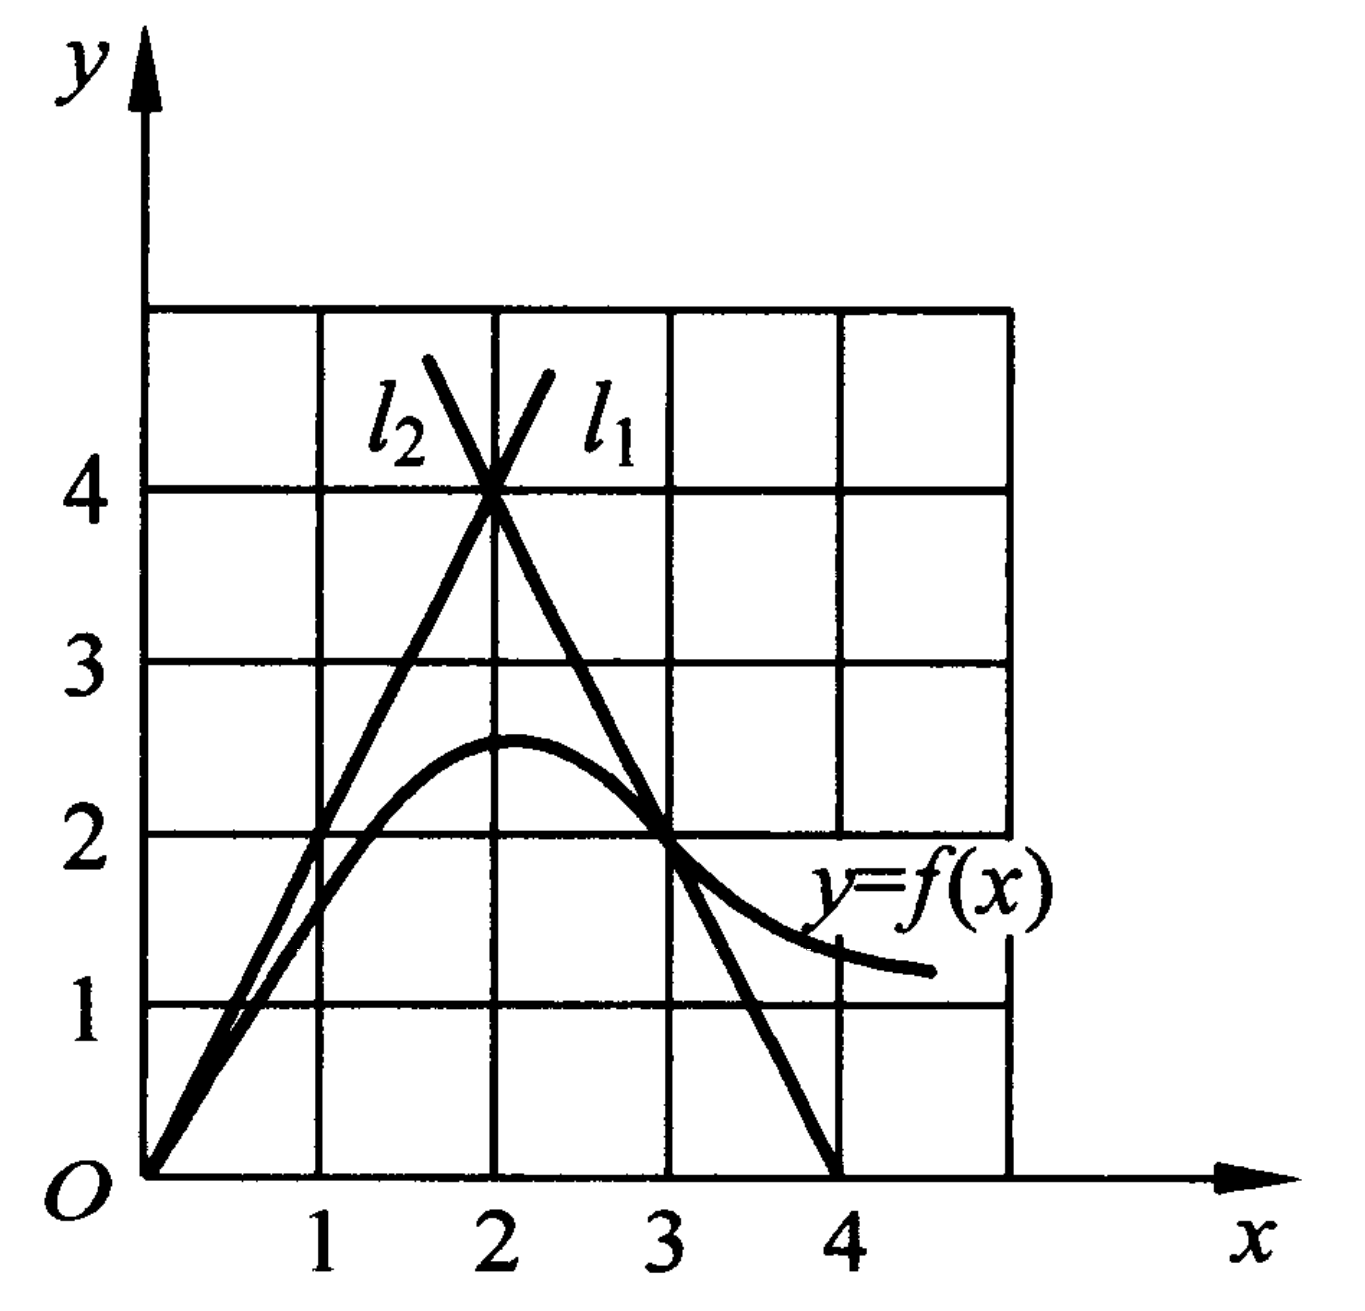
\includegraphics[width=0.5\linewidth]{image/P41-变式3.2-05_1,2.png}
\end{minipage}}
\ansat{263；【方法探究】 - 考点一 - 3.分部积分法 - 变式3.2}

% --- 题目 ---
\problem[P44-2 (21-3)]{设平面区域 $\displaystyle D$ 由曲线 $\displaystyle y=\sqrt{x} \sin \pi x$ ($\displaystyle 0 \le x \le 1$) 与 $\displaystyle x$ 轴围成, 则 $\displaystyle D$ 绕 $\displaystyle x$ 轴旋转所成旋转体的体积为 \underline{\hspace{4em}}.}
\ansat{263；【十年真题】 - 考点二 - 3.分部积分法 - 变式3.2}

\problem[P44-4 (23-2,3)]{已知平面区域 $\displaystyle D = \left\{(x,y) \left| 0 \le y \le \frac{1}{x \sqrt{1+x^2}}, x \ge 1 \right.\right\}$.
\begin{enumerate}
\item[(1)] 求 $\displaystyle D$ 的面积;
\end{enumerate}}
\ansat{267；【十年真题】 - 考点二：平面图形的面积与旋转体的体积 - 4}

% --- 题目 ---
\problem[P44-5 (20-2)]{设函数 $\displaystyle f(x)$ 的定义域为 $\displaystyle (0, +\infty)$ 且满足
$\displaystyle 2f(x) + x^2 f\left(\frac{1}{x}\right) = \frac{x^2+2x}{\sqrt{1+x^2}}. $
求 $\displaystyle f(x)$, 并求曲线 $\displaystyle y=f(x)$, $\displaystyle y=\frac{1}{2}$, $\displaystyle y=\frac{\sqrt{3}}{2}$ 及 $\displaystyle y$ 轴所围图形绕 $\displaystyle x$ 轴旋转所成旋转体的体积.}
\ansat{267；【十年真题】 - 考点二：平面图形的面积与旋转体的体积 - 5}

% --- 题目 ---
\problem[P44-6 (19-1,3-仅数学一、三)]{求曲线 $\displaystyle y=\mathrm{e}^{-x} \sin x$ ($\displaystyle x \ge 0$) 与 $\displaystyle x$ 轴之间图形的面积.}
\ansat{267；【十年真题】 - 考点二：平面图形的面积与旋转体的体积 - 6}

% --- 题目 ---
\problem[P52-1 (25-1)]{设函数 $\displaystyle f(x)$ 在区间 $\displaystyle [0, +\infty)$ 上可导, 则 ( \quad )
\begin{tasks}(1)
  \task 当 $\displaystyle \lim_{x \to +\infty} f(x)$ 存在时, $\displaystyle \lim_{x \to +\infty} f'(x)$ 存在.
  \task 当 $\displaystyle \lim_{x \to +\infty} f'(x)$ 存在时, $\displaystyle \lim_{x \to +\infty} f(x)$ 存在.
  \task 当 $\displaystyle \lim_{x \to +\infty} \frac{\int_0^x f(t)\mathrm{d}t}{x}$ 存在时, $\displaystyle \lim_{x \to +\infty} f(x)$ 存在.
  \task 当 $\displaystyle \lim_{x \to +\infty} f(x)$ 存在时, $\displaystyle \lim_{x \to +\infty} \frac{\int_0^x f(t)\mathrm{d}t}{x}$ 存在.
\end{tasks}}
\ansat{270；【十年真题】 - 考点二：含变限积分的函数的极限问题 - 1}

% --- 题目 ---
\problem[P52-7 (17-2,3)]{求 $\displaystyle \lim_{x \to 0^+} \frac{\int_0^x \sqrt{x-t} \, \mathrm{e}^t \, \mathrm{d}t}{\sqrt{x^3}}. $}
\ansat{271；【十年真题】 - 考点二：含变限积分的函数的极限问题 - 7}

% --- 题目 ---
\problem[P52-6 (19-2)]{已知函数 $\displaystyle f(x) = x \int_1^x \frac{\sin t^2}{t} \mathrm{d}t$, 则 $\displaystyle \int_0^1 f(x) \mathrm{d}x = \underline{\hspace{4em}}. $}
\ansat{272；【十年真题】 - 考点三：变限积分与其他问题的综合 - 6}

% --- 题目 ---
\problem[P53-8 (24-2)]{设 $\displaystyle t > 0$, 平面有界区域 $\displaystyle D$ 由曲线 $\displaystyle y=\sqrt{x} \, \mathrm{e}^{-x}$ 与直线 $\displaystyle x=t, x=2t$ 及 $\displaystyle x$ 轴围成, $\displaystyle D$ 绕 $\displaystyle x$ 轴旋转一周所得旋转体的体积为 $\displaystyle V(t)$, 求 $\displaystyle V(t)$ 的最大值.}
\ansat{272；【十年真题】 - 考点三：变限积分与其他问题的综合 - 8}

% --- 题目 ---
\problem[P53-10 (20-2)]{已知函数 $\displaystyle f(x)$ 连续且 $\displaystyle \lim_{x \to 0} \frac{f(x)}{x} = 1, g(x) = \int_0^1 f(xt) \mathrm{d}t$, 求 $\displaystyle g'(x)$ 且证明 $\displaystyle g'(x)$ 在 $\displaystyle x=0$ 处连续.}
\ansat{272；【十年真题】 - 考点三：变限积分与其他问题的综合 - 10}

% --- 题目 ---
\problem[P53-11 (16-2,3)]{设函数 $\displaystyle f(x) = \int_0^1 |t^2 - x^2| \mathrm{d}t$ ($\displaystyle x > 0$), 求 $\displaystyle f'(x)$, 并求 $\displaystyle f(x)$ 的最小值.}
\ansat{272；【十年真题】 - 考点三：变限积分与其他问题的综合 - 11}

% --- 题目 ---
\problem[P55-例5 (95-2)]{设 $\displaystyle f(x) = \int_0^x \frac{\sin t}{\pi - t} \mathrm{d}t$， 计算 $\displaystyle \int_0^\pi f(x) \mathrm{d}x$.}
\ansat{55；【方法探究】 - 考点三：变限积分与其他问题的综合 - 4. 求二次积分 - 例5}

% --- 题目 ---
\problem[P59-2 (18-2,3)]{设函数 $\displaystyle f(x)$ 在 $\displaystyle [0,1]$ 上二阶可导, 且 $\displaystyle \int_0^1 f(x) \mathrm{d}x = 0$, 则 ( \quad )}
\begin{tasks}(2)
  \task 当 $\displaystyle f'(x) < 0$ 时, $\displaystyle f\left(\frac{1}{2}\right) < 0$.
  \task 当 $\displaystyle f''(x) < 0$ 时, $\displaystyle f\left(\frac{1}{2}\right) < 0$.
  \task 当 $\displaystyle f'(x) > 0$ 时, $\displaystyle f\left(\frac{1}{2}\right) < 0$.
  \task 当 $\displaystyle f''(x) > 0$ 时, $\displaystyle f\left(\frac{1}{2}\right) < 0$.
\end{tasks}
\ansat{276；【十年真题】 - 考点三：不等式问题 - 2}